\chapter{Examples}
\label{sec:examples}
\INITIAL{T}{o construct useful examples} it is crucial that we consider both scenarios which are both likely to be encountered during a broad range of analysis scenarios, and specific enough to address the basic issues of visualizing unique types of data. The following use-cases discuss the aims of the analysis being suggested and how that relates to the anticipated patterns and visualizations discussed in the previous chapters. The generation of visualizations from an analyst's perspective is discussed, but details of how these are generated are left for Chapter 6.

%%%%%%%%%%%%%%%%%%%%%%%%%%%%%%%%%%%%%%%%%%%%%%%%%%%%%%%%%%%%%%%%%%%%%%%%%%%%
%%%%%%%%%%%%%%%%%%%%%%%%%%%%%%%%%%%%%%%%%%%%%%%%%%%%%%%%%%%%%%%%%%%%%%%%%%%%
\section{Census Data Analysis}
\label{sec:census}
\INITIAL{T}{he first case we will examine} is an analysis of data extracted from the United States census bureau database. This data set in particular has become a standard example data set used in statistical outlier detection, and particularly in the application and development of machine learning algorithms. It was extracted from the database in 1994, is available online in the University of California Irvine's machine learning repository \cite{Blake1998}, and was first used in publication in the paper "Scaling Up the Accuracy of Naive-Bayes Classifiers: a Decision-Tree Hybrid"\cite{Kohavi1996} in 1996. 

\paragraph{Demographic Data}
Demographic data provides a perfect example for most big data type analyses because it can be used in many fields with very little alteration to the methods applied. In social science or political research the study of individuals as would appear in a census is immediately applicable with obvious potential gains stemming from the results of the  analysis. Though the census itself may not necessarily be as interesting in the corporate world, capturing traits of individuals in a census is analogous to maintaining a database of employees or customers. Likewise any field which analyses individuals, whether they be medical patients or users of a mobile application, will apply similar if not identical methods to a data set of approximately the same semantic structure. 

\paragraph{Conditional Split}
In a machine learning context, this data set is used to predict whether the income of an individual exceeds \$50,000 per year. Because this data would normally be partitioned into a training and testing set for use with a predictive model such as a naive Bayes classifier or neural network, it includes a field with the correct response so that testing results can be verified. Thus, we already know whether an individual in the dataset falls into one of the two possible categories (>50K, <=50K) without analysis. We can therefore ignore any prediction and assume a much simpler data flow, a basic conditional split on the category field. If categorical demographic data is to be analyzed in an in-situ context, a reasonable question from an analyst who has not been able to prepare or pre-examine the data set in any rigorous way would be what proportion of records exist across the given categories. In cases where analysts have significant subject matter expertise, a simple visualization of these proportions would be enough to confirm expected results, show an unexpected reality, or imply an error in the quality of data or in the analysis methods.

\paragraph{Split Computation}
The actual MapReduce job for such a task is very simple, and consists of an implementation of the numerical summarization pattern. Firstly, the field containing the income categorization flag is extracted from the data source. Then, a flat map function returns a tuple for each record containing the income category and and the integer 1. Following this, we simply reduce by summing the "1" field across each category to determine the totals for each. This is analogous to the standard word count example paired with most MapReduce systems. To perform the visualization, only four lines of code must be added by the author of the analysis task, as seen below:

\paragraph{}
\begin{lstlisting}[language=Java,showspaces=false,showstringspaces=false,breaklines=true, breakatwhitespace=true]
        Visualizer visualizer = new Visualizer();
        InSituCollector totalsCollector = new InSituCollector(visualizer);
        totalsCollector.collect(1, totals, String.class, Integer.class);
        visualizer.visualizeBarChart(1, "Census Income Categories", "Category", "Count");
\end{lstlisting}

\paragraph{Visualization Code}
The first two lines create a visualizer and in-situ collector, respectively. The visualizer class doesn't require any parameters to be instantiated, and the collector requires a reference to the visualizer class so that it has somewhere to send collected data. The second two lines of code perform all of the actual work in visualizing the data from this flow. The collect method of the collector is called in the third line and accepts three arguments in this case. The first argument is an integer identifier for the collected data set, which can then be referenced later in order to specify which data is to be visualized. The second argument is a data set object from the Flink analysis task in question, and the remaining arguments are class objects representing the fields contained in the data set "totals", in order. In the last line, the actual visualization function is called from the visualizer. The first, and only required, argument to this function is the identifier of the data set which we collected earlier. Additionally, in this case three string arguments have been provided, which apply a title and axis labels to the resulting visualization. The resulting bar chart is shown in Figure \ref{fig:conditional}.     

%%%%%%%%%%%%%%%%%%
\begin{figure}
	\centering
	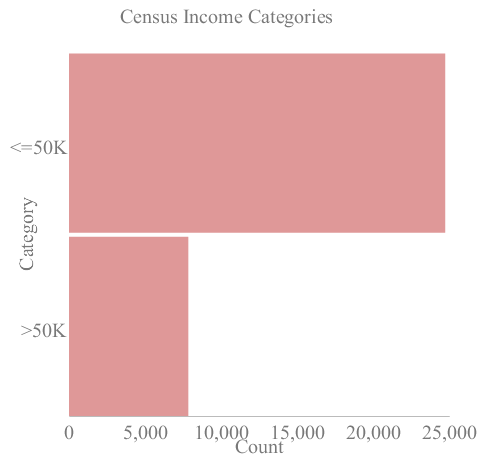
\includegraphics[scale=0.7]{Census_Conditional.png}
	\caption{A bar chart showing census income category proportions}
	\label{fig:conditional}
\end{figure}
%%%%%%%%%%%%%%%%%%

\paragraph{Bar Chart}
As discussed in Chapter 3, a bar chart is the most appropriate chart to be applied in the case of category comparison. We can see immediately when looking at Figure \ref{fig:conditional} that those who make less than \$50,000 are outnumbered by a rate of roughly 3:1 (in fact, the true proportion is 3.15:1). Given the limited input that is provided in the call to the visualizer, we achieve adequate results in the design of the chart. The labeling is clear and well formatted given the provided input. Even without the provision of labels from the method call, someone with an approximately accurate estimate about the outcome would be able to read the chart without labels. Of course, because we cannot know before the  program is run what values to expect, there are some limitations to the way in which we format the results. A good example of this is the x axis. If we desired axis value differences of less or more than 5,000 or a starting point other than 0 it is not a trivial change to make. However, because the purpose of this type of visualization is focused on getting a sense of data in the in-situ context rather than performing detailed visual analysis, it could be argued that such changes are unnecessary.

\paragraph{filtering}
With such a simple analysis task, it isn't unlikely that the developer performing the analysis would also perform some basic drill-down type analyses on the categories in question. In this case, we will filter each of the two income categories and split the records by age. It is of course expected that we will see some kind of trend from year to year in age, rather than strong variance over short sequences. As such, we will apply a line chart as opposed to another bar chart to visualize our expected approximately linear relationship. Figure \ref{fig:rich_line} shows the resulting line chart for our filtered set of high income earners. Semantically this shows us an interesting trend in the ages at which people seem to first reach a high income status, and conversely when they age into a lower bracket. More importantly however for an exploratory or in-situ analysis, we see that the data seems to make sense. "Spikes" in the line such as seen between age 40 and 60 are not dramatic enough to strongly indicate a problem in data quality, and in fact the overall bell curve shape of the plot indicates that the sample size for this data set  was large enough to reveal a pattern. Of course, a detailed analysis would be required to verify this with statistical significance but for exploratory purposes this is a good start. We can also compare this chart with the records from the opposite filter, as seen in Figure \ref{fig:poor_line}. This comparison allows us to identify interesting crossover points in the two trends that might be interesting for a detailed analysis. In this case, an interesting point for investigation might be around age 40 where a plateau exists for high earners and the trend for low earners is seemingly unaffected. 

%%%%%%%%%%%%%%%%%%
\begin{figure}
	\centering
	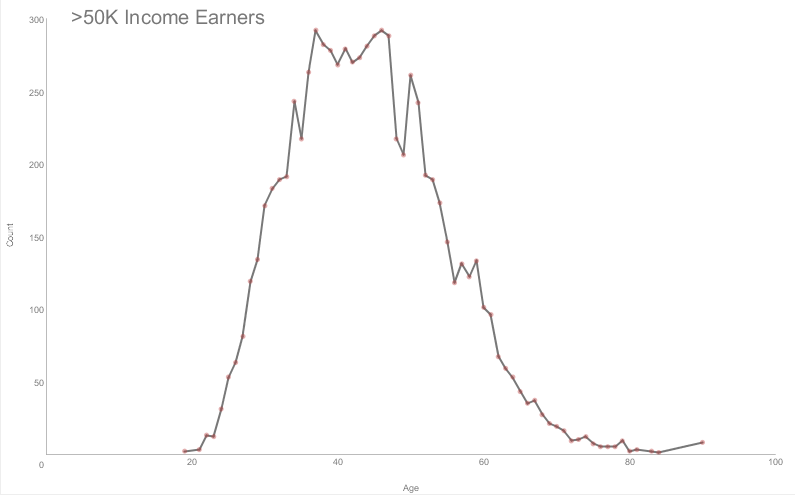
\includegraphics[scale=0.7]{rich_earners_line.png}
	\caption{A line chart showing the highest earners by age}
	\label{fig:rich_line}
\end{figure}
%%%%%%%%%%%%%%%%%%

%%%%%%%%%%%%%%%%%%
\begin{figure}
	\centering
	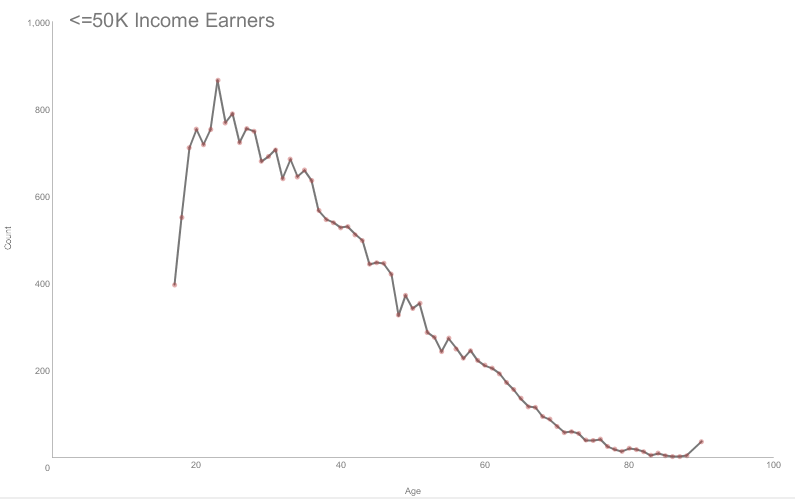
\includegraphics[scale=0.7]{poor_income_earners.png}
	\caption{A line chart showing the lowest earners by age}
	\label{fig:poor_line}
\end{figure}
%%%%%%%%%%%%%%%%%%

%%%%%%%%%%%%%%%%%%%%%%%%%%%%%%%%%%%%%%%%%%%%%%%%%%%%%%%%%%%%%%%%%%%%%%%%%%%%
%%%%%%%%%%%%%%%%%%%%%%%%%%%%%%%%%%%%%%%%%%%%%%%%%%%%%%%%%%%%%%%%%%%%%%%%%%%%
\section{Network Analysis}
\label{sec:network}
\INITIAL{N}{etwork data sets are ubiquitous} in many fields, as was briefly discussed in Chapter 3. We will examine some of the basic analyses identified by the KONECT project \cite{Kunegis2013}, and use the datasets they have provided in order to enable simple comparison of results and reproduction of visualizations which have been proven useful.

\paragraph{Les Misérables}
Firstly, we will examine a graph representing data extracted from the novel "Les Misérables" by Victor Hugo. Representing only a single work rather than a corpus of texts, this data set is relatively small. This enables us to examine the features of network data in general, and also those visualizations which relate to layout and will only be applicable with sufficiently few nodes. Within this network, each node represents a character in the narrative of the plot, and the edges represent a meeting between two characters. Each edge is weighted with an integer, representing the number of distinct times that the characters appear together. In summary, the graph is undirected and weighted.

\paragraph{Edge Weights}
Analyzing edge weights is one of the most common tasks that can be performed in network analysis. It is also one of the default analyses provided for all graphs within the KONECT data set, and has been replicated here in the same format to demonstrate that past useful results are replicable. The edge weight frequency graph as generated through this work is seen in Figure \ref{fig:edgeweightslesmis} and that avaiable through KONECT is seen in Figure \ref{fig:edgeweightskonect}. Each shows the distribution of edge weights in this graph, which in this case forms an approximately smooth decreasing curve. This is sensible for the graph in question, indicating that there are more character within Les Misérables who appear very infrequently, and thus encounter few other characters, than there are major characters for whom the opposite is true. In many situations, this kind of trend in edge weights may seem like an obvious conclusion, but there exist many scenarios where this is not the case beyond simply detecting errors in the data itself. 

%%%%%%%%%%%%%%%%%% 
\begin{figure}
	\centering
	\begin{minipage}{0.45\textwidth}
		\centering
		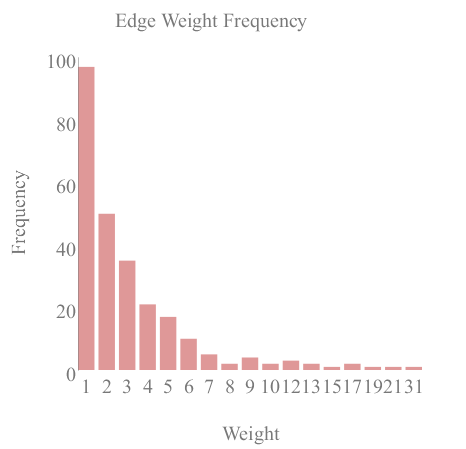
\includegraphics[scale=0.5]{edge_weights_lesmis_inverted.png}
		\caption{A bar chart showing edge weights in the Les Miserables network}
		\label{fig:edgeweightslesmis}
	\end{minipage}\hfill
	\begin{minipage}{0.45\textwidth}
		\centering
		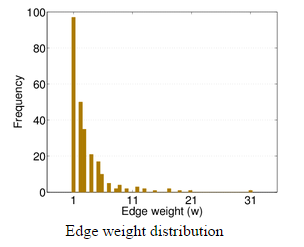
\includegraphics[scale=0.9]{konect_lesmis_edgeweight.png}
		\caption{A bar chart showing edge weights from KONECT}
		\label{fig:edgeweightskonect}
	\end{minipage}
\end{figure}
%%%%%%%%%%%%%%%%%%

\paragraph{Wikipedia Conflicts}
An example of a graph which displays a very different trend is the Wikipedia conflict graph \cite{konect:2014:wikiconflict}. This dataset was originally extracted for the purposes of examining structural similarities in social network graph data \cite{konect:brandes09}, and represents wikipedia users as nodes. Each edge in the graph represents an interaction between two users in conflict, an edit war being the typical example, with graph weights representing the nature of the interaction. Negative weights are associated with negative interactions, and the opposite for positive weightings. Examining Figure \ref{fig:wiki_conf} shows that we see an approximate bell-curve, with a gap in the center indicating that no neutral interactions were coded. It should be noted that due to the increase in the number of categories, the automatic formatting of the x-axis has caused the labels to run together somewhat, but the overall trend and important values are still easily identifiable. 

%%%%%%%%%%%%%%%%%%
\begin{figure}
	\centering
	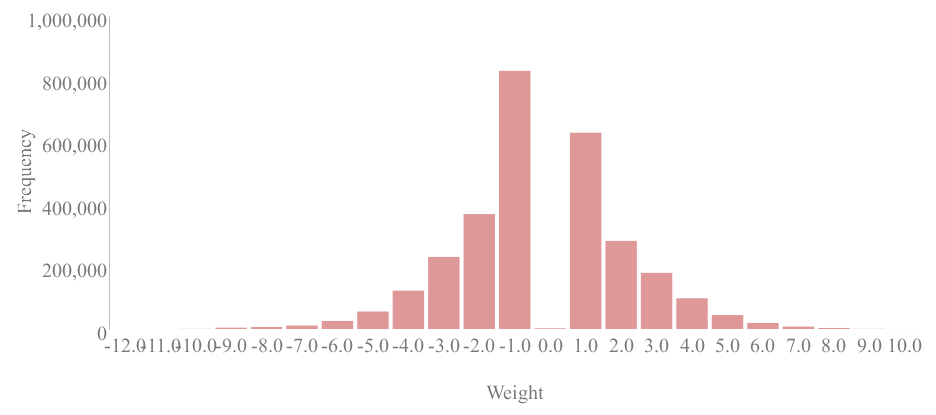
\includegraphics[scale=0.5]{conflict_edgeweights.png}
	\caption{A bar chart showing edge weight distribution in the wikipedia conflict graph}
	\label{fig:wiki_conf}
\end{figure}
%%%%%%%%%%%%%%%%%%

\paragraph{Degree Distribution}
Though edge weights are obviously specific to weighted graphs, there are other straightforward methods for assessing the structural elements of network data that apply to all graphs. A very common method of this is the calculation of degree distribution. Once again, a side by side comparison of the result generated by this solution and that given by KONECT is shown in Figure \ref{fig:degfreqlesmis} and Figure \ref{fig:degfreqlesmis} respectively. Here, the difference in the results of each visualization is stronger because of axis scaling. The KONECT visualization uses logarithmic scaling for both axes, but due to the general purpose design of the scatterplot visualization used in this work normal scaling is applied. Due to the limited size of this graph in particular normal scaling actually provides a clearer picture of where exactly points sit, but as the data set size is scaled up the number of points minimizes the effect that scaling has on legibility. 

%%%%%%%%%%%%%%%%%% 
\begin{figure}
	\centering
	\begin{minipage}{0.45\textwidth}
		\centering
		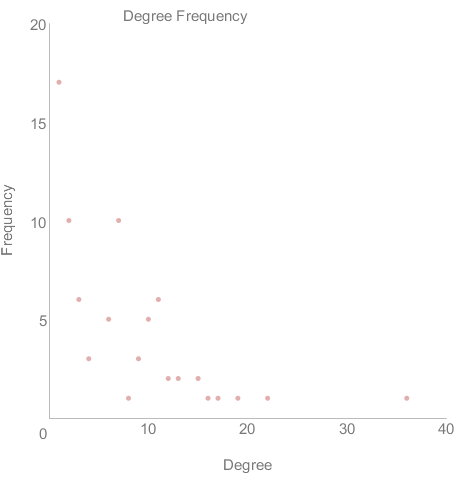
\includegraphics[scale=0.5]{degree_freq_lesmis.png}
		\caption{A scatter plot showing degree frequency in the Les Miserables network}
		\label{fig:degfreqlesmis}
	\end{minipage}\hfill
	\begin{minipage}{0.45\textwidth}
		\centering
		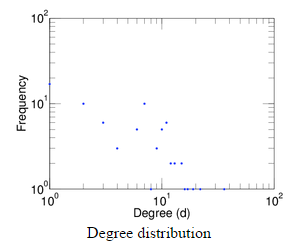
\includegraphics[scale=0.9]{konect_lesmis_degdist.png}
		\caption{A scatter plot showing degree frequency from KONECT}
		\label{fig:degfreqkonect}
	\end{minipage}
\end{figure}
%%%%%%%%%%%%%%%%%%

%%%%%%%%%%%%%%%%%%%%%%%%%%%%%%%%%%%%%%%%%%%%%%%%%%%%%%%%%%%%%%%%%%%%%%%%%%%%
%%%%%%%%%%%%%%%%%%%%%%%%%%%%%%%%%%%%%%%%%%%%%%%%%%%%%%%%%%%%%%%%%%%%%%%%%%%%
\section{Classification}
\label{sec:classification}
\INITIAL{A}{s one of the core tasks in exploratory data mining} classification provides a scenario which would very likely rely on in-situ data processing. The data set to be examined is the "Iris Plants Database" \cite{Fisher1936} which first appeared in 1936 as an example of discriminant analysis. It consists of four measurements: the width and length of both the petal and sepal of three different species of iris. Based on its initial use in developing a model which distinguished different iris species, it has since been used as a standard test case for various classification techniques. If this data is examined from the perspective of an analyst with limited prior knowledge of the features of the data (apart from the species included) visualizations can be used to limit potential classification methods. 

\paragraph{Scatter Plot}
A basic visualization of this data such as in Figure \ref{fig:sepal_clustering} immediately indicates that there are two distinct clusters in the data set.  Additionally, it can be seen that some of the points in the scatter plot have darker colouring than others. This indicates identical records in the source data set, with darker points indicating more duplicates. Because axis scaling is based on the values present in the data set rather than some pre-determined range, they are well distributed across the layout of the plot at the expense of what is arguably an unorthodox axis origin. The two cluster shown isolate on of the three species in the data set, but do not separate the remaining two visually. This is somewhat interesting, but is limited in that only two variables are seen at once, perhaps hiding some relationship that exists between another combination of our iris features. As we expect three classes of data within the set, it follows that we should hope to see three approximately separate clusters in one such comparison.

%%%%%%%%%%%%%%%%%%
\begin{figure}
	\centering
	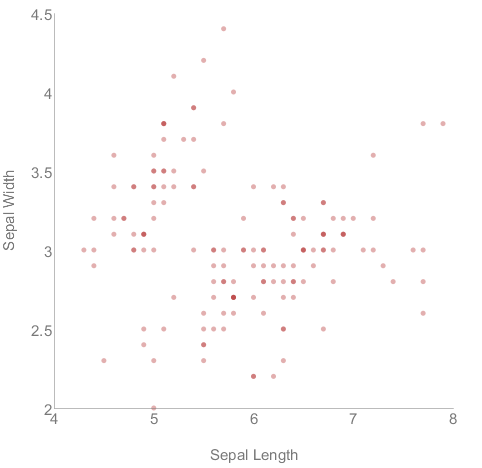
\includegraphics[scale=0.7]{sepal_clustering.png}
	\caption{A scatterplot showing iris sepal data}
	\label{fig:sepal_clustering}
\end{figure}
%%%%%%%%%%%%%%%%%%

\paragraph{Matrix Plot}
A standard method for examining the relationship between multiple variables is to simply visualize each combination in a grid, in this case as a scatter plot matrix. Such a visualization can be seen in Figure \ref{fig:scatterplot_matrix}. While the fine grain details in such a visualization are somewhat more obscured in comparison to the individual scatter plot, we can now easily obtain an approximate idea of the relationships between each variable in our data set. The matrix is composed of a square grid with dimensions equal to the number of variables to be compared, with the main diagonal of the grid representing the variables themselves. The remaining squares in the matrix are filled with scatter plots; where the x-axis of each represents the variable with which it shares a column, and the y-axis the variable with which it shares a row. The relative size of the plots will of course be scaled to the number of variables present, but may be impractical with larger numbers of variables. The labeling and titles are less important here as we are focused on broad visual patterns more than specific statistic, similar to the case with spark lines. Also, because labels for the variables do not exist in the Flink data set being analyzed in this case, placeholder names are given to each variable. It is assumed that either the user is aware of the order in which they were provided to the collector and can infer their semantic meaning, or that the specific variable names themselves are unimportant relative to the patterns exhibited.

\paragraph{Classification Method}
In this case, we can see that across all plots in the matrix only two clearly demarcated clusters exist. This means that regardless of which variables are chosen for comparison, we are unlikely to be able to separate all three species of iris using a simple linear method. An analyst faced with such a figure would be likely to apply a supervised learning method if at all possible, or perhaps a more complex unsupervised method such as a linear principal component analysis. 

%%%%%%%%%%%%%%%%%%
\begin{figure}
	\centering
	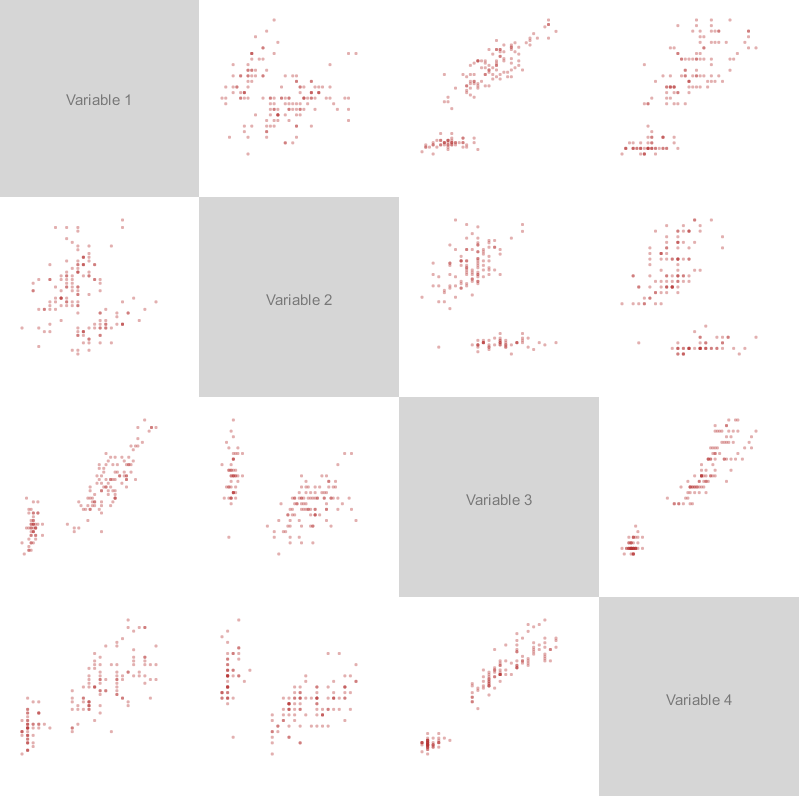
\includegraphics[scale=0.7]{scatterplot_matrix.png}
	\caption{A scatterplot matrix showing iris data across all variables}
	\label{fig:scatterplot_matrix}
\end{figure}
%%%%%%%%%%%%%%%%%%